\input{/home/haldean/Documents/latex_template.tex}
\title{Simulated Volumetric Displays using Head Tracking}
\begin{document}
\maketitle

My project seeks to create a program that simulates a volumetric
display by tracking the user's head and modifying the image displayed
on the screen to mimick parallax perspective. 

\section{Volumetric Displays}
Volumetric displays (devices capable of three-dimensional video
output) have long been relegated to the realm of science fiction;
until recently, volumetric displays existed only in imaginations. In
late 2009, Sony unveiled the world's first feasible volumetric display
at the DC Expo in Tokyo \citep{sonydisplay}. This device was capable
of a resolution of 98 by 98 by 128-pixel resolution, and the
cylindrical display was 13 centimeters in diameter. Today, two and a
half years later, consumers are still waiting for volumetric displays
to come to market, and while we are seeing a rise in 3D-television
adoption, there seem to be very little demand for holographic or other
kinds of volumetric displays.

On the other hand, simulated volumetric displays (or ``parallax
displays'') like the one I plan on building have seen quite a few
recent and not-so-recent implementations, with various success. Some
rely on specialized hardware, such as Johnny Lee's implementation
which uses a Wiimote as a camera and infrared LEDs mounted on glasses
to determine the user's location in 3D space \citep{wiiproject}. Other
systems, mostly for using head motions as input to videogames, use
tracking markers that are worn on a baseball cap. I was unable to find
a popular implementation that did not utilize tracking markers, but
there are published papers that suggest that it has been done, and
with good results. I discuss this software and research in Section
\ref{sec:sources}.

\section{Motivation}
I want to create a volumetric display because it has interesting,
practical uses and is relatively simple to implement, given the
libraries available. It also is something that is fun for an end-user
to use, and easy to integrate into other software. I've found the
available software either heavily platform-dependent (usually
dependent on a Windows system), closed source, or difficult to use for
anything other than very basic, demonstrative purposes. If this
project goes well, I would like to turn it into a cross-platform
library for building parallax display into other 3D software after the
end of the semester. 

There are many possible use cases, but I thought of this project idea
when working on my 3D printer. I spend lots of my time modelling
objects for 3D printing, and having the ability to really ``look'' at
an object on a convincing, three-dimensional display before it is
printed would have saved me many reprints.

\section{Relevant Software and Research}
\label{sec:sources}
\begin{description}
\item[VR Displays using Wiimotes] A similar project has been done by
  Johnny Lee, in which he displayed visual output that was modified
  based on head position to simulate a 3D display. However, he used a
  Wiimote to track the user's head; the user wore glasses with
  infrared LEDs attached, and a Wiimote then communicated the
  location, rotation and distance of the glasses to the computer. He
  has released the source code for program he uses to do the head
  tracking \citep{wiiproject}; it is written in C\# and uses the
  Win32 API.

\item[VR for Videogames: Cachya] Cachya \citep{cachya} is a system
  designed to translate head location and pose into joystick or mouse
  events for use in videogames. It is primarily used as input for
  flight simulators, but could potentially be used in other games as
  well. Cachya uses a webcam system, but requires the user to wear a
  tracking marker on a hat. There is a very involved calibration step,
  as well, in which the user has to directly manupulate various image
  parameters (contrast, brightness, threshold, etc.) before they can
  use the system. Even after all of this calibration, a significant
  amount of smoothing is then done to prevent noisy input, which would
  be detrimental to a videogame. It uses machine learning techniques
  to attempt to identify the threshold between noise and input.

\item[VR for Videogames: TrackIR] Another major player in the
  videogame head tracking market is TrackIR \citep{trackir}. This
  system uses a specialized camera and an marker device to track the
  user's head. While the technology behind the camera is proprietary,
  it does seem to be an infrared camera, perhaps with some sort of
  structured light emission, as the marker device is reflective. It
  has six degrees of freedom, just like Cachya: roll, pitch, yaw, pan
  horizontally, pan vertically, and depth. Calibration is optional,
  and allows the user to change the response to various kinds of
  motion; for example, a user can select how sensitive the system
  should be to movements in different axes.

\item[Head-Tracking Libraries] The Enhanced Human-Computer Interface
  library \citep{ehci} is a library designed for real-time head
  tracking in three dimensions. It has six degrees of freedom, and
  outputs a 3-vector normal to the plane of the face. It was designed
  for a parallax display application, but then was changed for more
  general-purpose usage; it now exists only as a system designed for
  adding head-based gestural control to other applications.

\item[Review of Head-Tracking Methods] An older paper,
  \citep{parallax}, discusses various methods of face detection that
  his team tested in creating a parallax system not unlike my
  own. They tested five methods: foreground segmentation, color-based
  tracking, motion-based tracking, facial detection and a Baysian
  network that simulates a combination of all tracking of the
  previously mentioned methods. They found that the motion-based
  system performed the best of any individual method, but the Baysian
  network outperformed that method by a significant amount.

\item[Review of Gesture Recognition Techniques] A more recent paper,
  \citep{eyetracking}, proposes various algorithms for detecting
  hands, noses and eyes in images. The various methods of detecting
  eyes that are described could be very useful, as interocular
  distance could serve as an accurate measurement of depth. However,
  the outlined algorithms are also much more difficult to implement
  than just a standard face detection algorithm; if I find that facial
  detection is giving poor results, I will try some of the algorithms
  given here.
\end{description}

\section{Implementation Details}
I have two different methods in mind for how to implement face
detection, both of which were proposed in \citep{parallax}. One is a
segmentation based on color, and is not dissimilar from the
segmentation method used in the first assignment. The other is a
motion-based system, which evaluates the location of the face based on
changes in pixel values. The color-based method assumes that the
lighting of the face doesn't change and there are few skin-colored
objects in the room, while the motion-based method assumes that
nothing else in the frame is moving. I plan on implementing both of
these methods to determine which gives me the best results, and then
using that method going forward.

Once I have the bounding box of the face, I will then use the centroid
of the face and it's size along the primary axis of the bounding
rectangle to detect approximate relative location in three
dimensions. After applying some smoothing, I will use the location in
reference to the center of the frame (which I assume to be aligned
with the center of the display) to determine the perspective from
which the user would be viewing the scene.

At first, the system will be capable of some basic parallax using
layers of images. This mode of operation will require the user to
input various images and the ``depth'' at which each image lies. The
location of the user's head will then be used to displace those images
in relation to each other to create the appearance of multiple image
planes with differing depth.

The next step will be to integrate the parallax system with
OpenGL. Instead of a series of images, the system will read in a 3D
scene from a descriptor file. The user moving their head will
correspond to movements within this 3D scene. 

\section{Feynstein Integration}
For my Programming Languages and Translators course, my team is
designing a language for physical simulation called Feynstein. This
language takes as input a description of a scene with objects and
forces, and outputs a visual simulation of that scene in a window on
the user's computer. If I have time after building my system as
outlined above, I would like to integrate my volumetric display with
the output of the Feynstein system. This would be completely optional,
and this system integration would not be presented for a grade in
Visual Interfaces.

\section{System Evaluation}
It is simple to come up with qualitative methods for judging the results
of the system; after all, this is a system designed to simulate the
physical phenominon of parallax perspective. If the simulated third
dimension is convincing to the user, and the image does appear to have
depth, I would consider the project a success. 

However, there are some qualitative measures I can use as well. The
metric I will monitor is jitter in the perceived head location, which
I anticipate will be a problem. I can log the location and depth of
the face on each measurement, then fit a polynomial function to the
results. If we assume that the user keeps their head relatively
steady, the average error between the measured values and the
polynomial will be equivalent to the error in the detected face
location. This will be a good test of whether or not my facial
detection and smoothing algorithms are working well.

\section{Sample Output}
Figures \ref{fig:facecenter}, \ref{fig:faceleft}, and
\ref{fig:facecorner} show some sketches of the sort of output I would
expect. On the left of each image is a ``webcam capture'',
representing where the user's face lies in relation to the scene. On
the right is a sample rendering of how a cube would be displayed, if
the user's face was in the corresponding location.

\begin{figure}
  \centering
  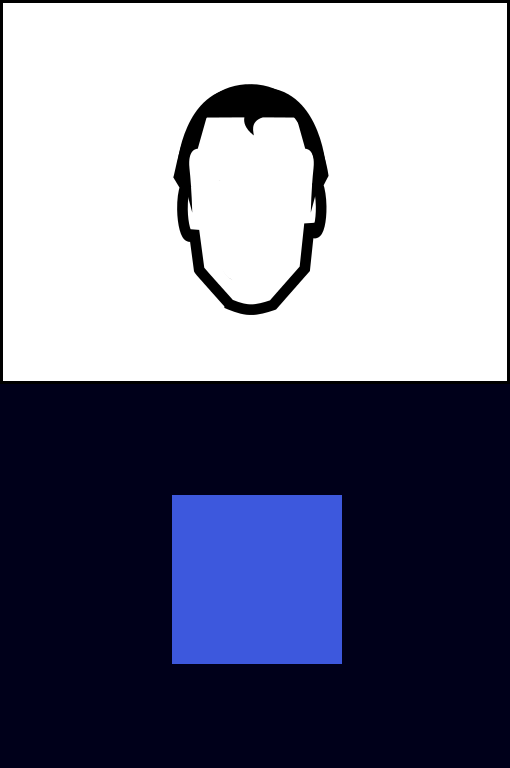
\includegraphics[scale=0.3]{images/head-center}
  \caption{The user's face is centered, so they see the front
    projection of the cube.}
  \label{fig:facecenter}
\end{figure}

\begin{figure}
  \centering
  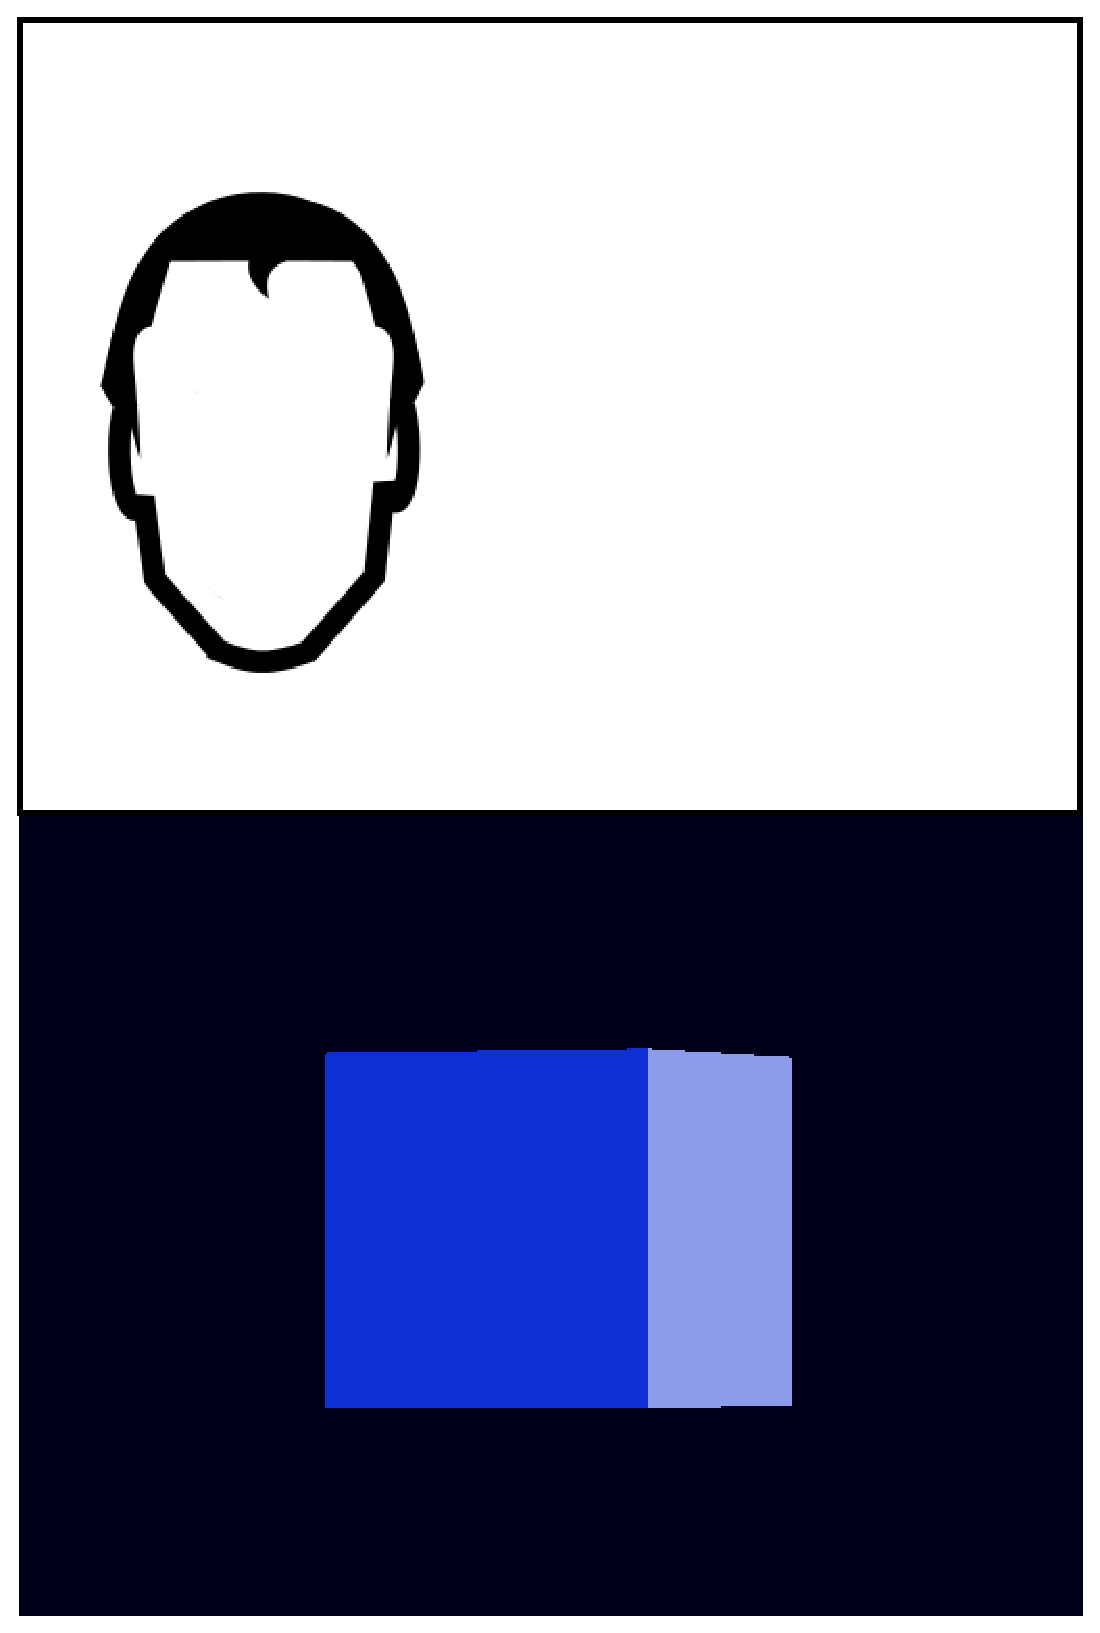
\includegraphics[scale=0.3]{images/head-left}
  \caption{The user's face is on the left, so they see the cube from
    the right.}
  \label{fig:faceleft}
\end{figure}

\begin{figure}
  \centering
  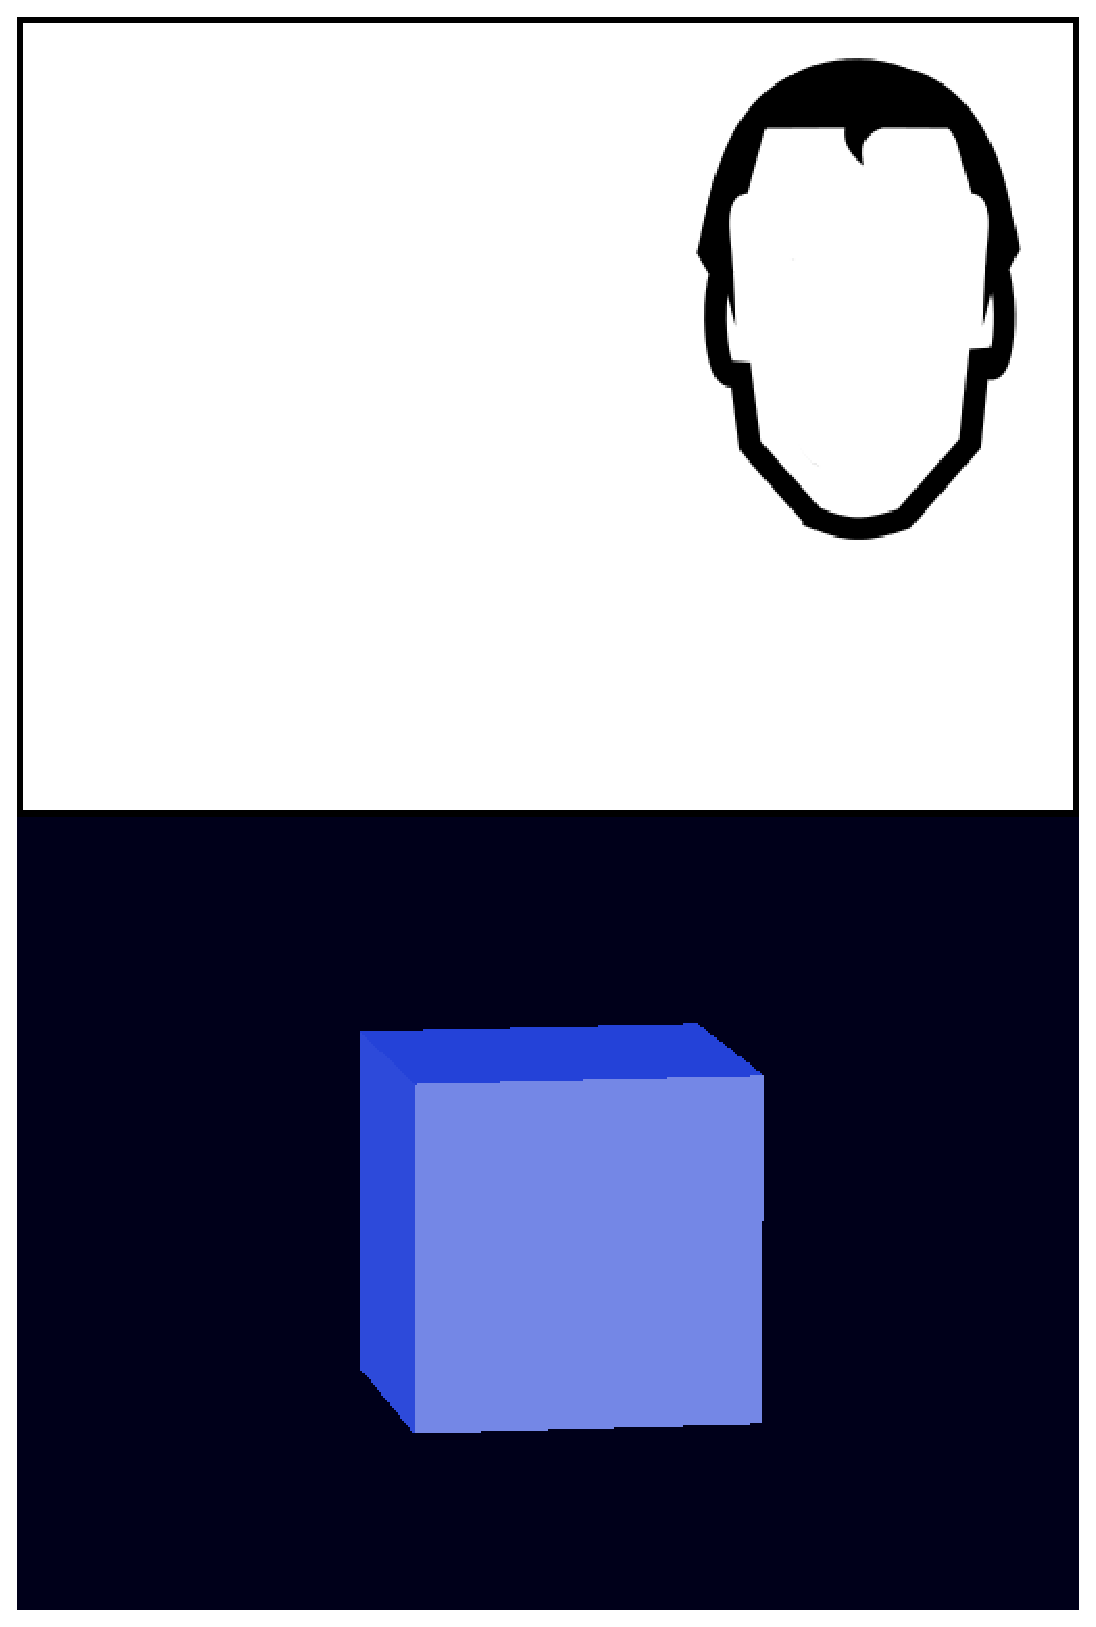
\includegraphics[scale=0.3]{images/head-corner}
  \caption{The face is in the top-right, so the cube is seen
    from the left and above.}
  \label{fig:facecorner}
\end{figure}

\begin{figure}
  \centering
  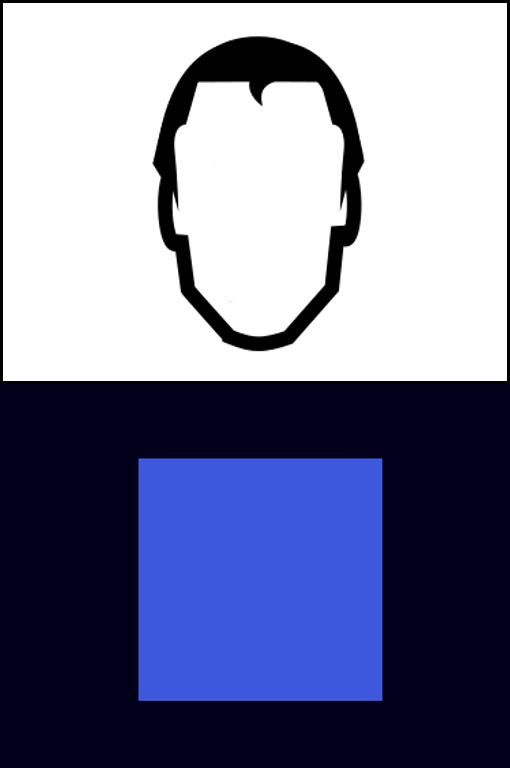
\includegraphics[scale=0.3]{images/head-close}
  \caption{When the user moves closer, the scene zooms in.}
  \label{fig:faceclose}
\end{figure}

\bibliographystyle{plainnat}
\bibliography{proposal}

\end{document}